La rappresentazione schematica del dispositivo di Foucault si trova rappresentata in figura (\ref{Pro}), prima di lato, poi dall'alto focalizzandosi sulle componenti presenti sul banco ottico tra la sorgente del laser e lo specchio rotante.
Come sorgente luminosa S è stata utilizzata una sorgente laser, in modo da risolvere il problema posto al termine del paragrafo precedente: la sua luminosità è molto alta (abbastanza da risultare molto fastidiosa ad osservazione diretta), pertanto il raggio di ritorno risulta visibile nonostante il piccolo rapporto R. Per evitare danni all'osservatore durante la preparazione dell'apparato, è stata utilizzata una coppia di lamine polaroid da porre tra il fascio luminoso e il punto di osservazione per ridurre l'intensità luminosa del laser.
\begin{figure}[htp!]
  \centering
  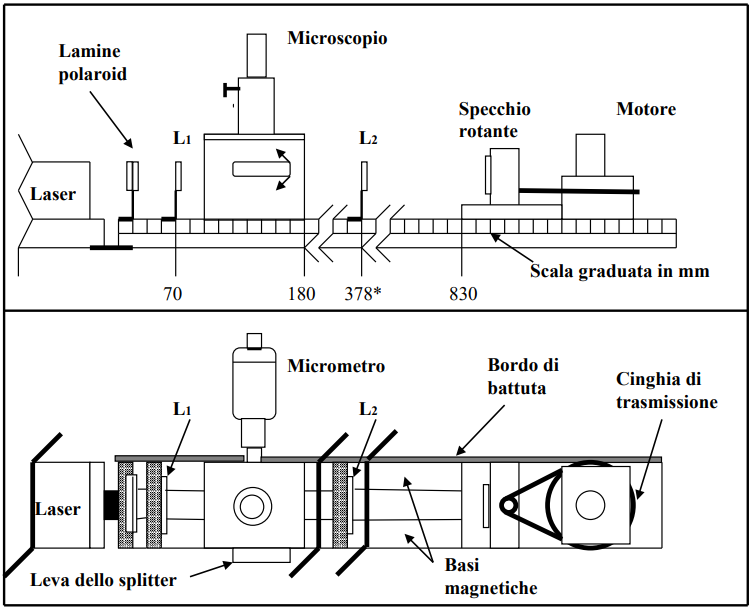
\includegraphics[scale=0.5]{Immagini/Apparato.png} 
  \centering
  \caption{Dalla seguente immagine si può visualizzare schematicamente l'apparato sperimentale in due prospettive: la vista laterale e dall'alto in modo da comprendere con maggiore dettaglio le varie componenti.}
  \label{Pro}
\end{figure}
Le lenti $L_1$, di distanza focale $f_1=48mm$, e $L_2$, di distanza focale $f_2=252mm$ (entrambe le misure note con un'incertezza $\sigma_f=1mm$) sono poste tra il laser e lo specchio rotante per garantire che la sorgente rimanga puntiforme durante tutta la distanza in quanto il laser, a lunghe distanze diventa un fascio di luce divergente. I supporti delle lenti sono dotati di magneti in grado di ancorarli con una certa stabilità alle basi magnetiche poste lungo il banco ottico. L'asse delle lenti può essere leggermente traslato poiché anche le lenti sono magneticamente attaccate ai loro supporti.

Tra le due lenti viene inserito un supporto che include lo splitter e il microscopio.
Lo splitter è una superficie di vetro semiargentata, orientata in modo da indirizzare il fascio luminoso di ritorno nel cannocchiale, posto in verticale perpendicolarmente al piano e al di sopra dello splitter. Per garantire ciò, la superficie semiriflettente deve essere la seconda ad essere attraversata dal raggio luminoso uscente dalla sorgente.

Sia il supporto delle lenti che dello splitter devono essere posizionati contro il bordo di battuta e durante l'esperienza occorre assicurarsi che non ruotino per evitare che si perda precisione nel posizionamento dei componenti.

Lo specchio rotante è collegato attraverso una cinghia di trasmissione ad un motorino, ed è regolabile la frequenza della sua rotazione mediante un dispositivo che presenta:
\begin{itemize}
    \item un interruttore di accensione (ON-OFF),
    \item un interruttore per la scelta del senso di rotazione (CW-CCW),
    \item una manopola per aumentare e diminuire gradualmente la frequenza di rotazione,
    \item un display che mostra la frequenza di rotazione,
    \item un pulsante che permette di portare la frequenza al massimo raggiungibile (circa 1500 giri al secondo) per un tempo massimo di 60 secondi,
    \item una luce rossa che indica un surriscaldamento o un problema del dispositivo e che invita a spegnere l'apparato se rimane acceso per più di 5 secondi.
    

\end{itemize}
Per allungare il più possibile la distanza D tra lo specchio rotante e lo specchio concavo, sono stati utilizzati gli specchi piani $S_1$ ed $S_2$ che permettono in uno spazio ridotto di raddoppiare le lunghezze in gioco. Per ultimo, Lo specchio concavo $M_f$ completa l'apparato sperimentale, riflettendo il raggio luminoso e dando origine al fascio di ritorno.
\begin{figure}[htp!]
  \centering
  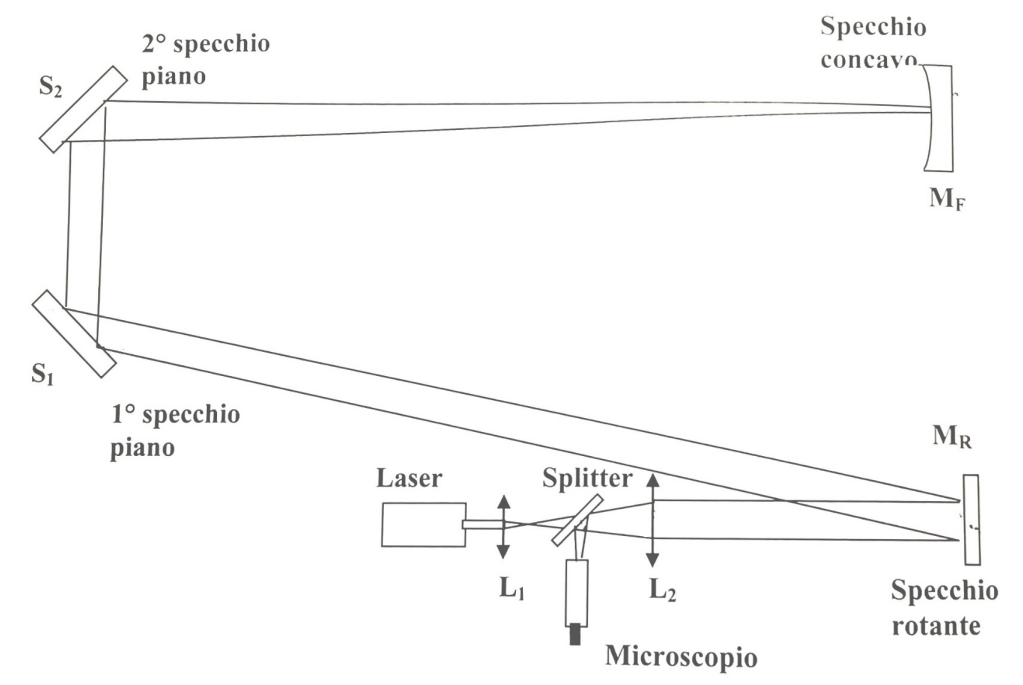
\includegraphics[scale=0.4]{Immagini/Apparato sperimentale.png} 
  \centering
  \caption{Nella seguente immagine si può osservare in modo schematico l'apparato sperimentale e il percorso che il fascio di luce laser compie durante l'esperimento.}
  \label{App}
\end{figure}
